\documentclass[tikz]{standalone}
\usepackage{pgfplots}
\usepackage{pgffor}
\usepackage{tikz-3dplot}
\usepgfplotslibrary{fillbetween}
\usepgfplotslibrary{patchplots}
\usetikzlibrary{3d}
\usepgfplotslibrary{colorbrewer} 
\tikzset{
  jumpdot/.style={mark=*,solid},
  excl/.append style={jumpdot,fill=white},
  incl/.append style={jumpdot,fill=black},
}
\usetikzlibrary{arrows.meta,intersections,calc,quotes,angles}
\pgfplotsset{width=7cm,compat=1.18} 
\begin{document}
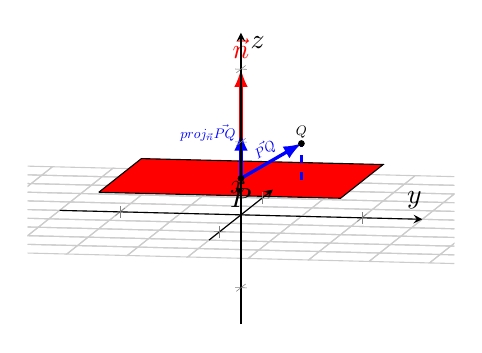
\begin{tikzpicture}
\begin{axis}[
  axis lines=center, 
  grid=major,
  axis on top,
  xmin=-3,
  xmax=3,
  ymin=-3,
  ymax=3,
  zmin=-3,
  zmax=5,
  xlabel=$x$,
  ylabel=$y$,
  zlabel=$z$,
  view={80}{-10},
  %%xtick={-3,0,...,5},
  %%ytick={-5,0,...,5},
  %%ztick={0,3,...,15},
  xticklabel = \empty,
  yticklabel = \empty,
  zticklabel = \empty,
]

%xy grid lines
\addplot3[mesh, gray!40, samples=11, samples y=11, forget plot] {0};
\addplot3[fill=red] coordinates {
  (-2,-2,1)
  (-2,2,1)
  (2,2,1)
  (2,-2,1)
  (-2,-2,1)
};
\draw[red,-latex,very thick] (0,0,1) -- (0,0,4) node[above] {$\vec{n}$};
\draw[blue,dashed,very thick] (0,1,1) -- (0,1,2) node[above] {};
\draw[blue,-latex,very thick] (0,0,1) -- (0,1,2) node[midway,above,sloped,scale=.5] {$\vec{PQ}$};
\draw[blue,-latex,very thick] (0,0,1) -- (0,0,2.25) node[left,scale=.5] {$proj_{\vec{n}}\vec{PQ}$};

\draw plot [mark=*, mark size=1,white] coordinates{(0,0,1)} node[below,scale=1] {$P$};
\draw plot [mark=*, mark size=1,blue] coordinates{(0,1,2)} node[above,scale=.5] {$Q$};
\end{axis}
\end{tikzpicture}
\end{document}